\chapter{Implementation and Application Workflows}
\section{From Architecture to a Working Assessment}
The recovery mechanism is integrated with an application that teachers and learners can use. A teacher prepares and publishes a classroom assessment; a learner enters it, answers against a server-managed attempt, and receives a submission reference. These operations exercise authentication, authorisation, persistence, grading, and recovery through the same public API.

The screens in this chapter were captured from the running application on 23 October 2026 using a synthetic BCSE355L classroom and a five-question, fifteen-minute assessment~\cite{local-capture}. They show local mode: two backend HTTP servers share an in-memory store within one process. They establish the implemented user workflow; the separate AWS experiment in Chapter~6 supplies evidence for cloud recovery.

\begin{figure}[H]\centering
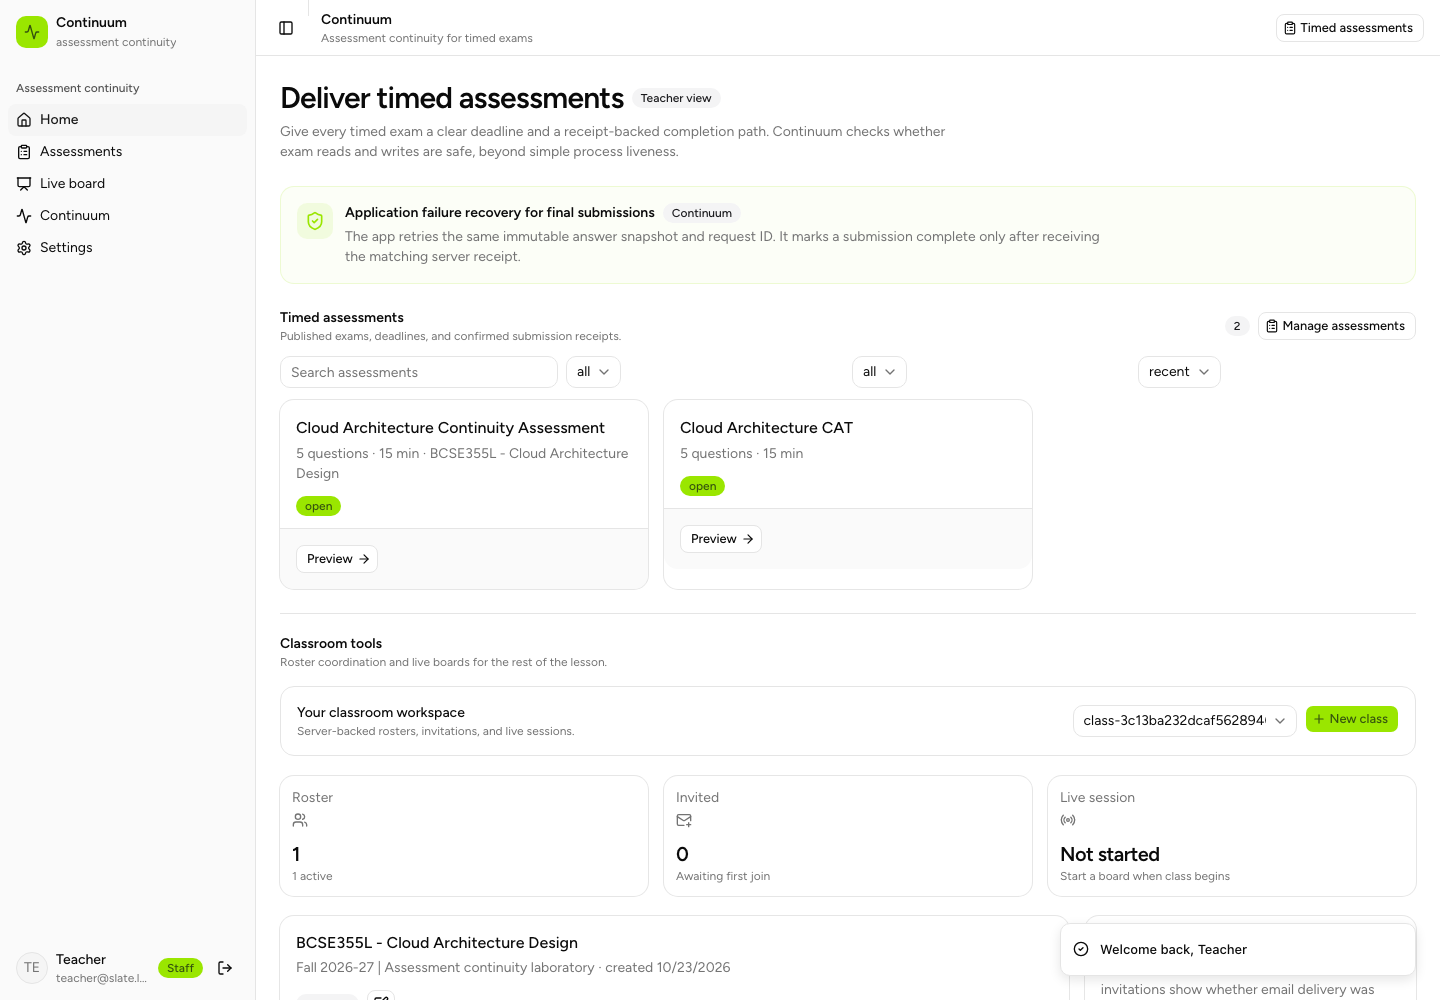
\includegraphics[width=\textwidth,trim=265bp 230bp 15bp 60bp,clip]{screenshots/teacher-dashboard.png}
\caption[Teacher home and classroom overview]{Teacher home with classroom context and assessment actions, using synthetic course data.}\label{fig:teacher-home}
\end{figure}

\Needspace{10\baselineskip}
\section{Teacher Preparation and Publication}
The editor captures the title, classroom, instructions, duration, and attempt limit. Each question has options, a correct choice, points, and feedback. The example uses five two-point questions, making the maximum score ten.

A draft permits preparation before learners see the assessment. Publishing exposes it through the catalogue. Published questions are protected against changes to an existing grading basis; availability and instructions remain separately managed~\cite{project-source}.

Classroom membership and API role checks protect assessment access and management. Retakes create a new attempt context while preserving earlier receipts.

\begin{figure}[H]\centering
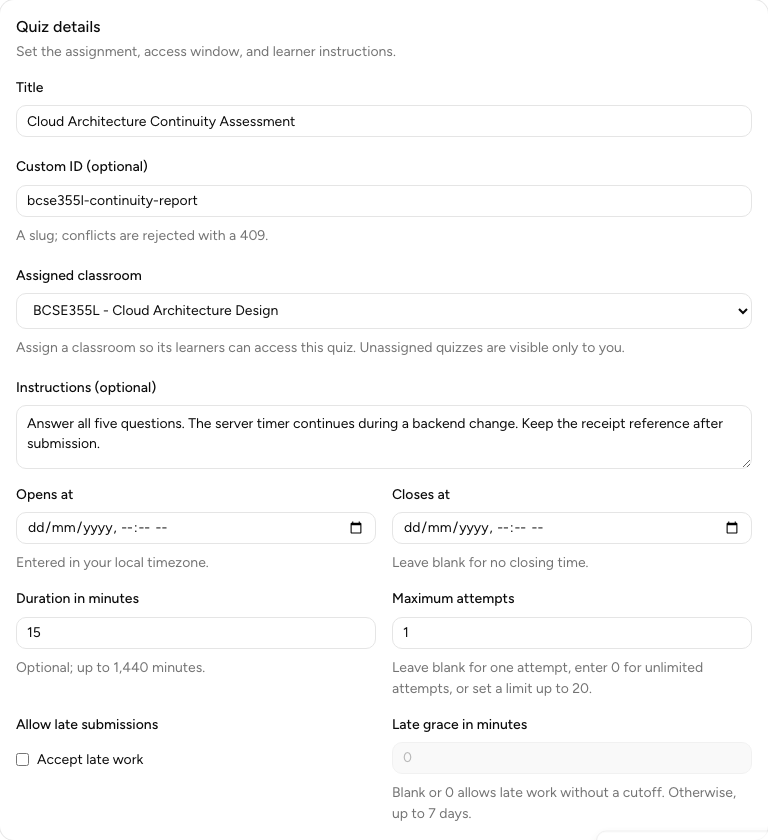
\includegraphics[width=125mm]{screenshots/teacher-assessment-settings.png}
\caption[Assessment policy settings]{Assessment policy: classroom assignment, instructions, a fifteen-minute duration, and one allowed attempt.}\label{fig:teacher-policy}
\end{figure}

\begin{figure}[H]\centering
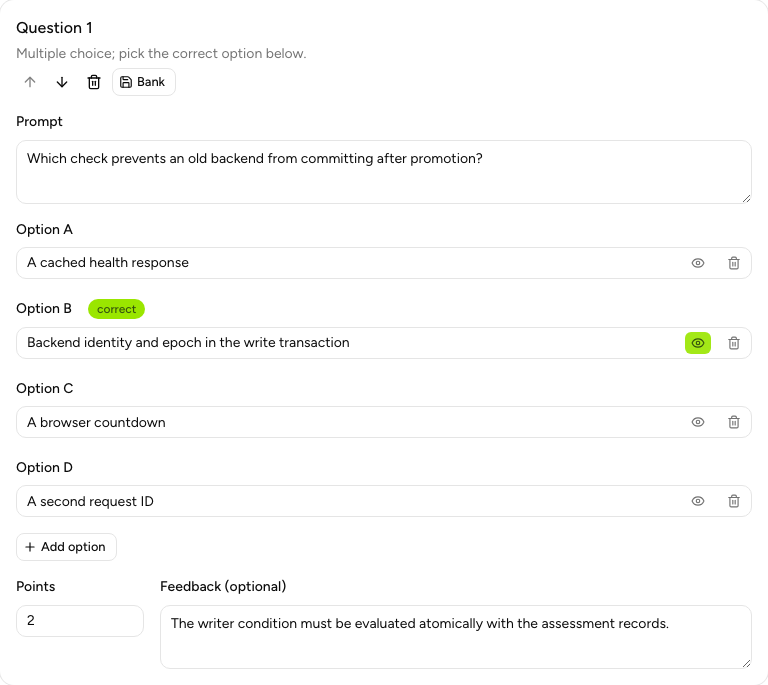
\includegraphics[width=125mm]{screenshots/teacher-question-editor.png}
\caption[Question authoring and grading configuration]{Question authoring with a selected correct option, explicit points, and explanatory feedback.}\label{fig:question-editor}
\end{figure}

\begin{figure}[H]\centering
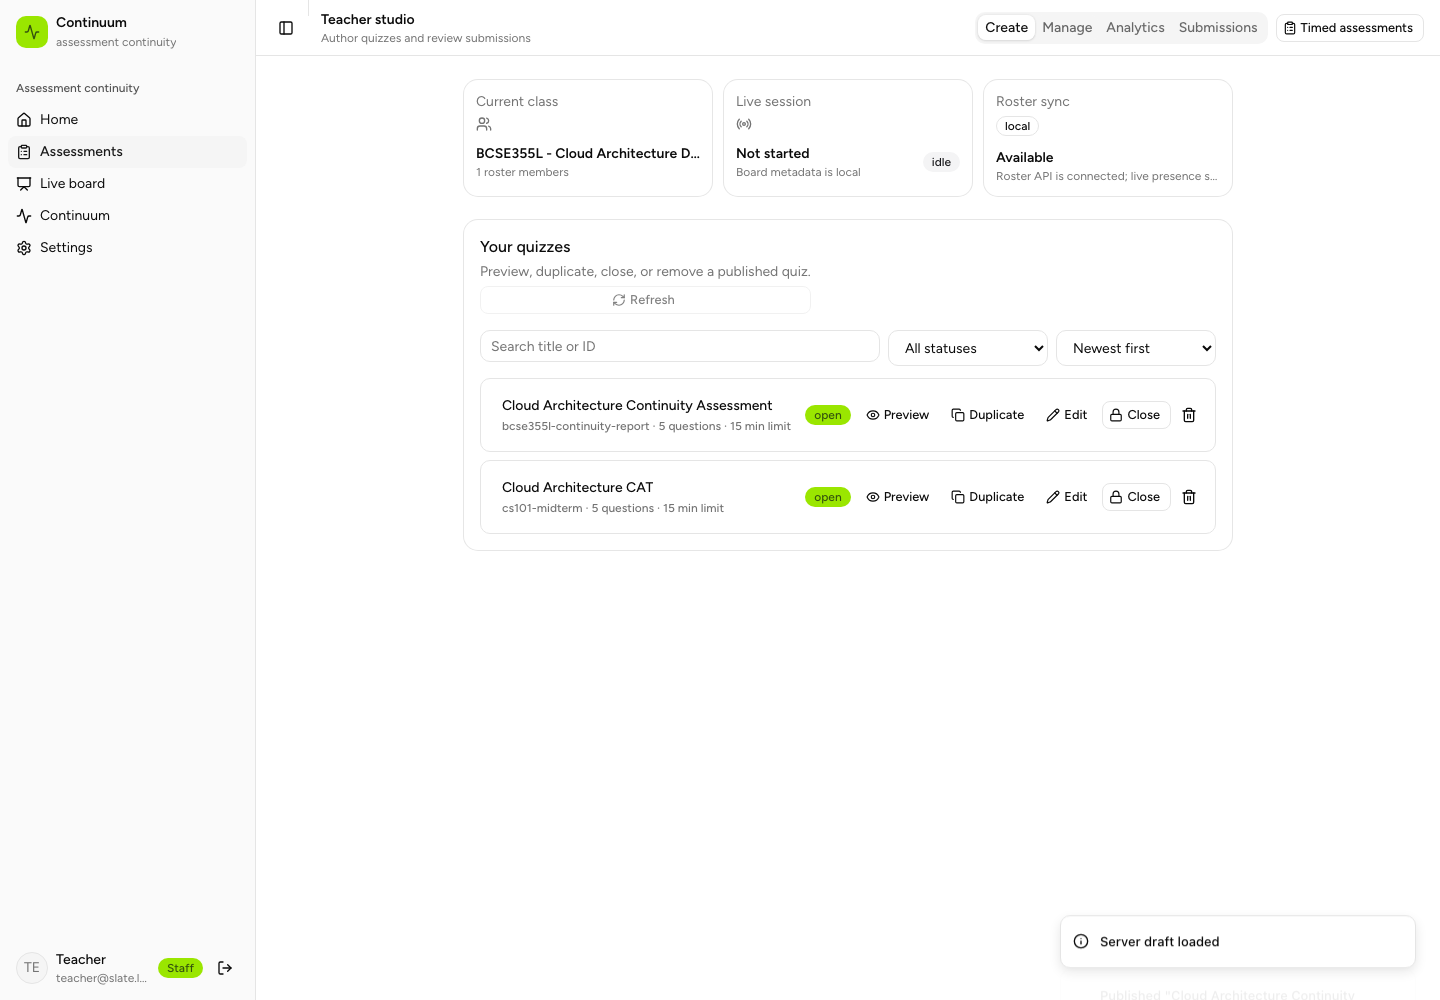
\includegraphics[width=150mm,trim=430bp 430bp 140bp 65bp,clip]{screenshots/teacher-published-assessment.png}
\caption[Published assessment management]{Teacher management view after publication, with availability and lifecycle controls.}\label{fig:published}
\end{figure}

\FloatBarrier
\section{Learner Entry and Timed Answering}
After authentication, the learner sees assessments permitted by classroom membership. The catalogue supports discovery; the lobby explains the selected assessment before the learner starts. Starting obtains the server-managed attempt and its persisted start time. Changing backend does not create another start event.

\begin{figure}[H]\centering
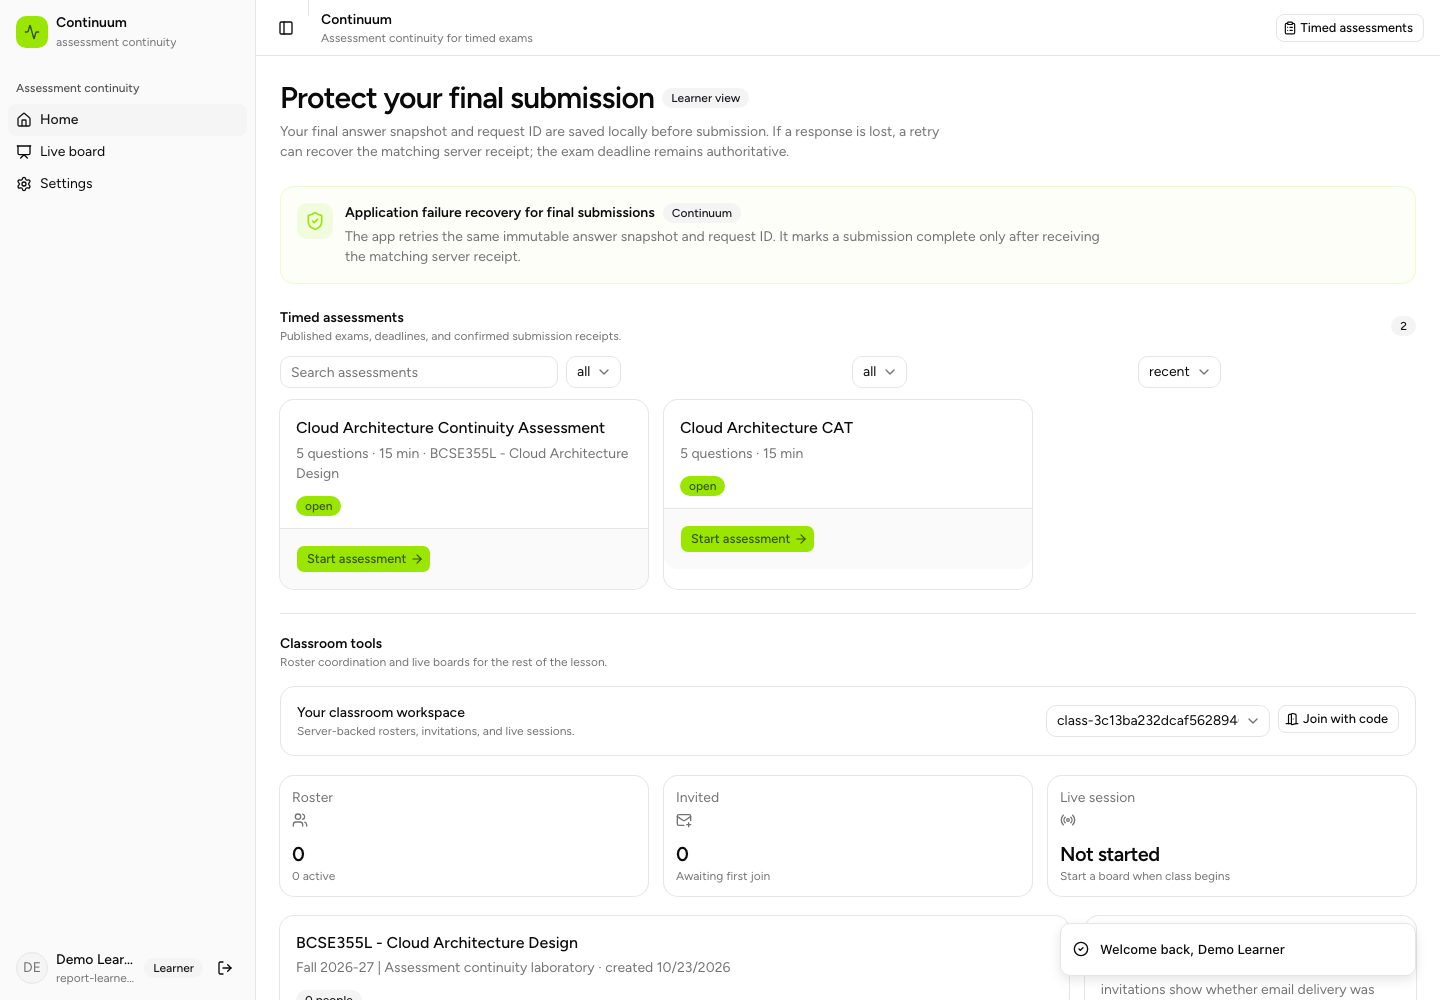
\includegraphics[width=\textwidth,trim=265bp 390bp 15bp 60bp,clip]{screenshots/learner-assessment-catalog.png}
\caption[Learner assessment catalogue]{Learner catalogue containing the published Cloud Architecture Continuity Assessment.}\label{fig:catalogue}
\end{figure}

\begin{figure}[H]\centering
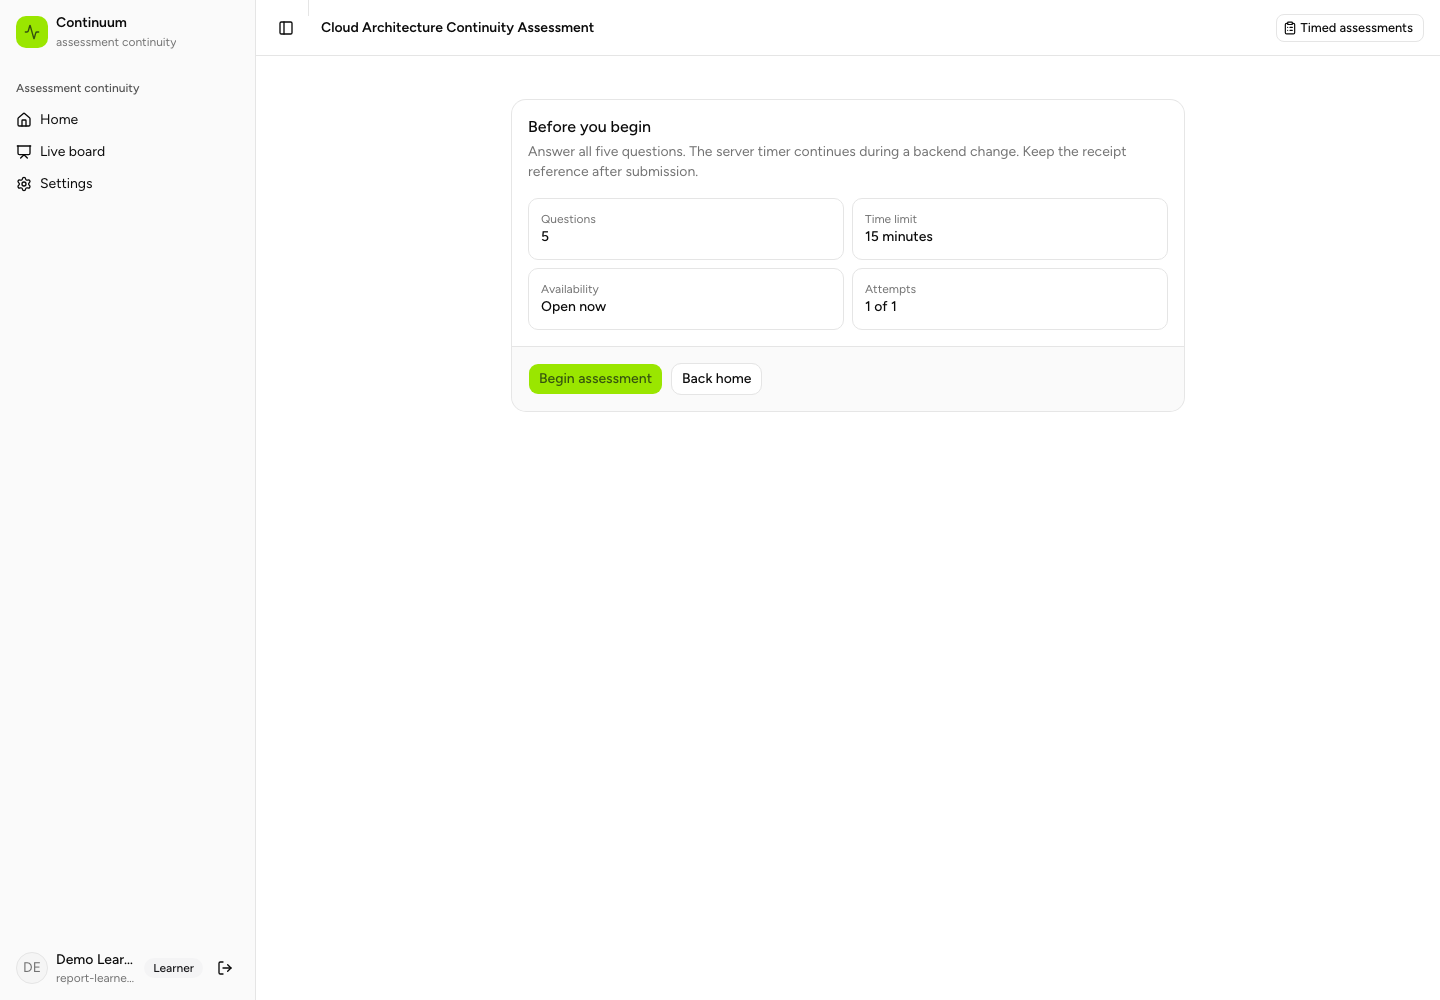
\includegraphics[width=\textwidth,trim=480bp 560bp 220bp 85bp,clip]{screenshots/learner-assessment-lobby.png}
\caption[Assessment lobby and start policy]{Assessment lobby showing instructions and the policy before the timed attempt begins.}\label{fig:lobby}
\end{figure}

\Needspace{5\baselineskip}
Within the assessment, navigation separates answering from review. A learner can select an answer, flag a question, revisit unanswered questions, and inspect the remaining time before submission. These controls help the learner identify what remains to be done without creating a second attempt during an interruption.

\begin{figure}[H]\centering
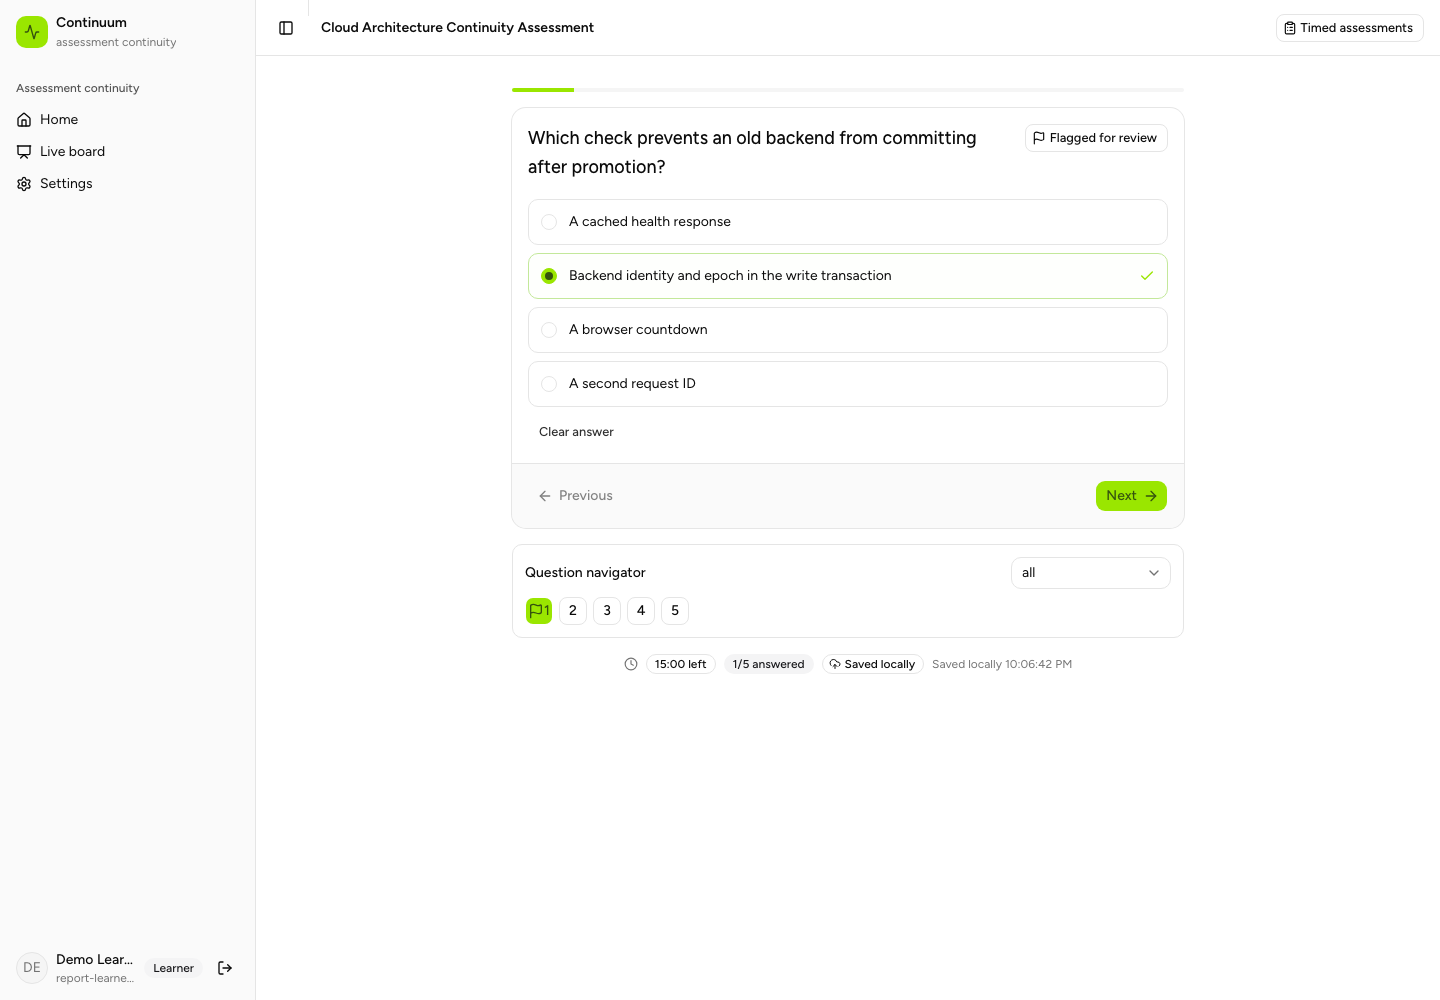
\includegraphics[width=\textwidth,trim=480bp 300bp 220bp 75bp,clip]{screenshots/learner-answer-and-review.png}
\caption[Timed answering and review controls]{Timed answering with a selected choice, review flag, question navigation, remaining time, and local-save status.}\label{fig:answer-review}
\end{figure}

\subsection{Three Different Meanings of Saved}
Browser storage, acknowledged progress, and a committed final result are separate states. ``Saved locally'' means this browser retained progress; a successful save response acknowledges backend attempt state. Only a final receipt identifies the immutable submitted snapshot and committed outcome.

Figure~\ref{fig:resume} demonstrates continuation from device state, rather than durability after browser loss. Backend changes preserve the attempt start time. Its deadline also depends on the current duration setting; Section~\ref{sec:timing-policy} explains that policy boundary.

\begin{figure}[H]\centering
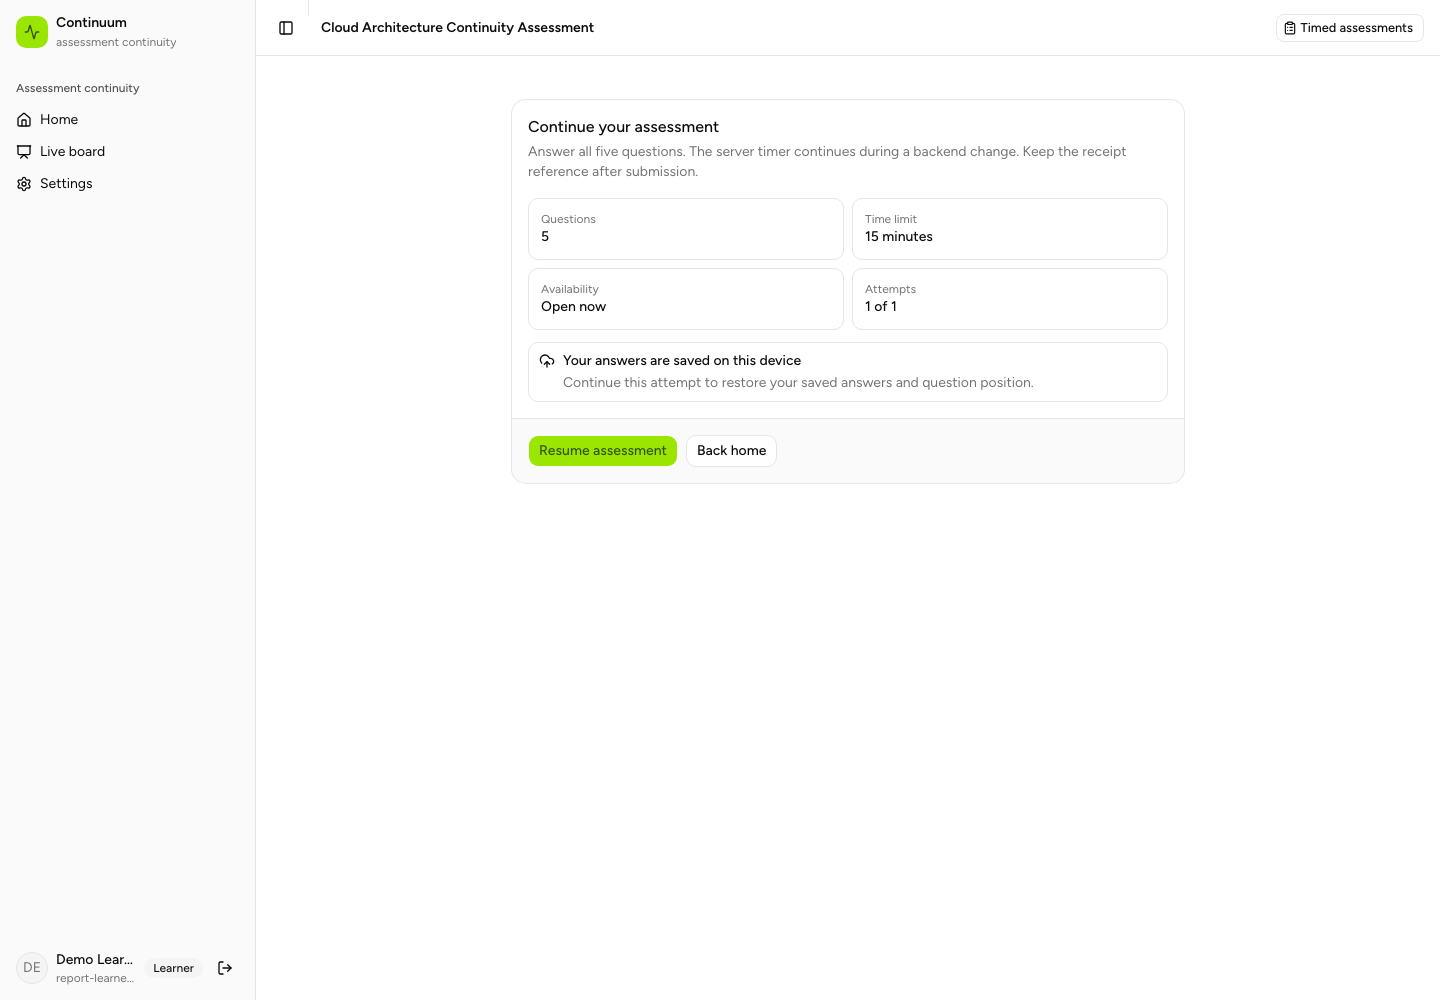
\includegraphics[width=150mm,trim=480bp 500bp 220bp 85bp,clip]{screenshots/learner-resume-attempt.png}
\caption[Continuing a saved attempt]{Continuation prompt after revisiting the assessment. The interface identifies answers retained on this device.}\label{fig:resume}
\end{figure}

\FloatBarrier
\section{Final Submission and Receipt Retrieval}
Before final submission, the browser preserves a request identifier with a fixed answer snapshot. Bounded retries use this identity rather than generating a different logical submission for every network attempt. A transport error may leave the outcome unknown, so the interface resolves the receipt before asking the learner to create a new submission.

Figure~\ref{fig:local-receipt} shows the completed synthetic attempt: score, submission time, receipt reference, copy/download actions, and question feedback. This local capture illustrates receipt retrieval through the application. It is not the response-loss experiment; equality of the original and replayed AWS commit is established independently in Chapter~6.

\begin{figure}[!htbp]\centering
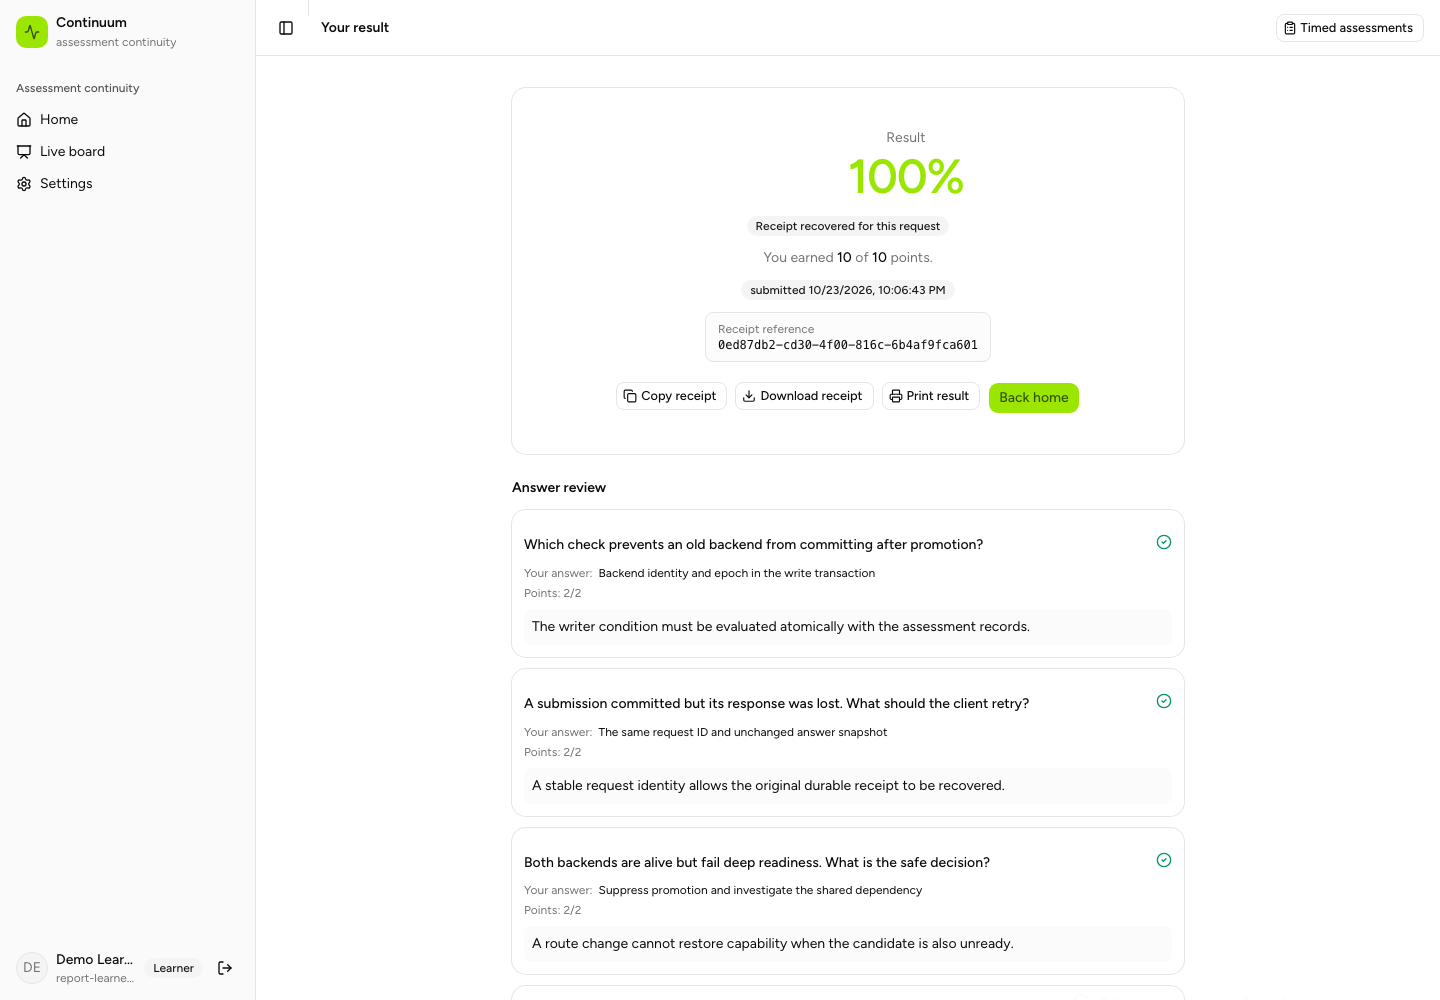
\includegraphics[width=150mm,trim=480bp 320bp 220bp 75bp,clip]{screenshots/learner-committed-receipt.png}
\caption[Retrieved local submission receipt and feedback]{Retrieved local result with a receipt reference, submission time, and answer review. The synthetic learner earned ten of ten points.}\label{fig:local-receipt}
\end{figure}

\section{Code Structure and Deployment}
Go implements the backend; React and TypeScript implement the interface. TanStack Router and Query coordinate navigation and server state, while Vite and Tailwind CSS support the frontend build. The AWS implementation uses the Go SDK v2 and Terraform. Table~\ref{tab:modules} identifies the boundaries that make the recovery contract reviewable.

\begin{table}[htbp]\centering\small
\caption{Implementation boundaries and the contracts they protect}\label{tab:modules}
\begin{tabularx}{\textwidth}{@{}L{53mm}Y@{}}\toprule
\textbf{Source boundary} & \textbf{Responsibility}\\\midrule
\path{internal/httpapi} & Authentication, classroom access, validation, and response mapping\\
\path{internal/exams} & Availability, attempt timing, saving, retakes, and submission rules\\
\path{internal/store} & Memory/DynamoDB persistence; receipts, attempts, transactional writes\\
\path{internal/clusterstate} & Authoritative backend/epoch contract for protected writes\\
\path{internal/continuum} & Router, capability probes, monitoring, control state, and events\\
\path{cmd/demo-reconciler} & Conditional outbox processing and audit completion\\
\path{statemachine/demo-failover.asl.json} & Recovery sequence, verification, and error paths\\
\path{infra/demo} & Supported single-Region AWS deployment\\
\path{web/src} & Role workflows, pending requests, and receipt presentation\\\bottomrule
\end{tabularx}\end{table}

Build scripts package application and Lambda artifacts deterministically. Bootstrap retrieves a private bundle and encrypted runtime configuration. A full deployment can replace instances and therefore requires a maintenance window. Pause/resume preserves the desired instance and monitoring state; private deployment files remain outside the report package.
